\begin{frame}{Lærkepletter}

\small

\begin{columns}[T]

\begin{column}{0.58\textwidth}

\textbf{Regler for lærkepletter:}

\begin{itemize}[]
\item Mindst 16 m²
\item Min. 2 per hektar
\item Mindst 40 m til kanten af marken
\item Må ikke gødskes eller sprøjtes
\end{itemize}

\vspace{0.4em}

\textbf{Gavner arter:}

\footnotesize
Sanglærke, bomlærke, vibe, agerhøne, markpiber, agerpistol, gul vipstjert, 
rødrygget tornskade, gulspurv, vilde bier, humlebier, dagsommerfugle, 
rovbiller, græshopper, musvåge, tårnfalk

\end{column}

\begin{column}{0.40\textwidth}
\centering
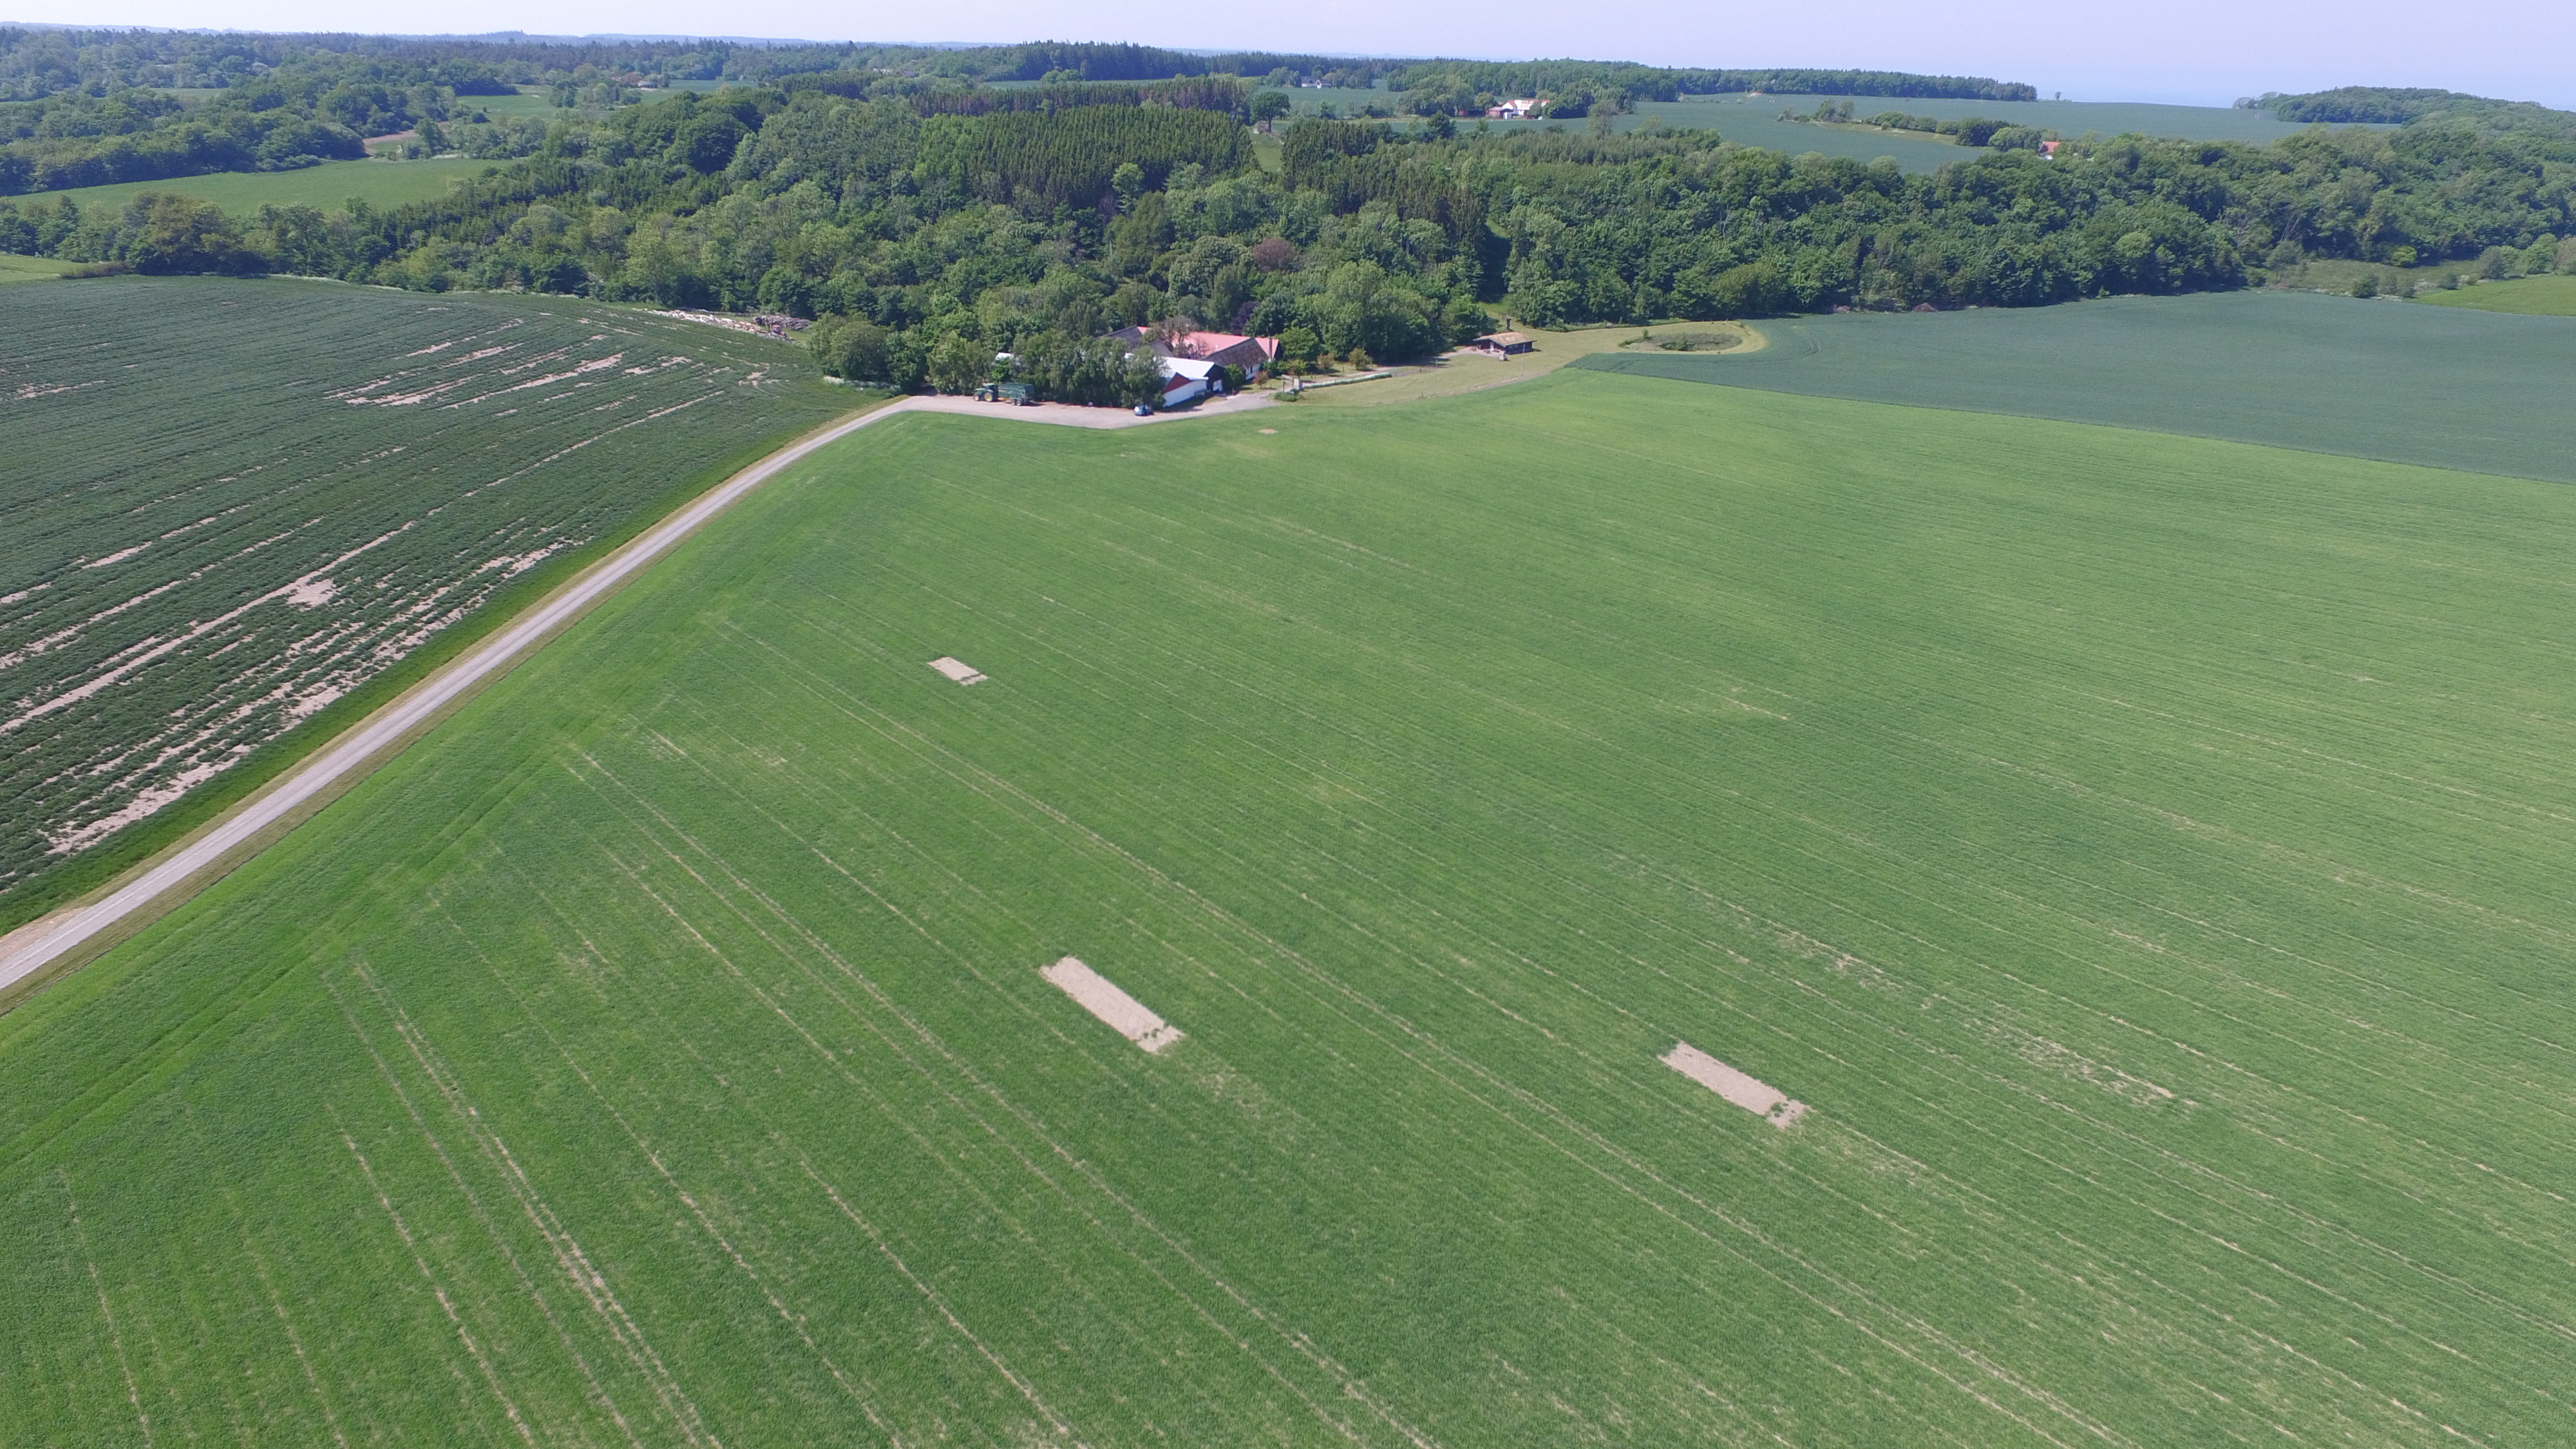
\includegraphics[width=\textwidth]{Billeder/Vildtforvaltning/biotopplantiltag/lærkepletter.jpeg}
\end{column}

\end{columns}

\end{frame}